\begin{abox}
	Electronics
	\end{abox}
\begin{enumerate}
	\item The circuit is as shown in figure
	\begin{figure}[H]
		\centering
		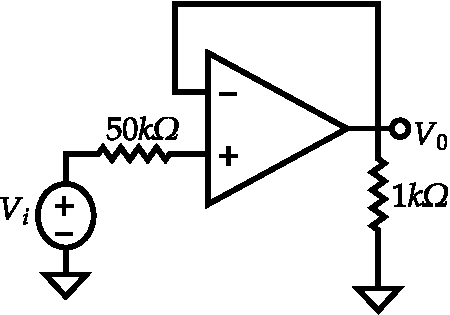
\includegraphics[height=3cm,width=4.5cm]{CE-1}
	\end{figure}
	(i) The ideal closed loop voltage gain is
	 \begin{tasks}(4)
		\task[\textbf{a.}]1
		\task[\textbf{b.}]$-1$
		\task[\textbf{c.}]$\infty$
		\task[\textbf{d.}]50 
	\end{tasks}
	\begin{answer}
		$$
		\begin{aligned}
		\text { Voltage follower circuit, } V+&=V_{i}, V-=V_{i}=V_{0}, \frac{V_{0}}{V_{i}}=1 \text {. Hence, (a) is correct answer. }\\
		\end{aligned}
	$$
	\end{answer}
	\item The op-amp of figure has a very poor open-loop voltage gain of 45 but is otherwise ideal. The closed loop gain of amplifier is
	\begin{figure}[H]
		\centering
		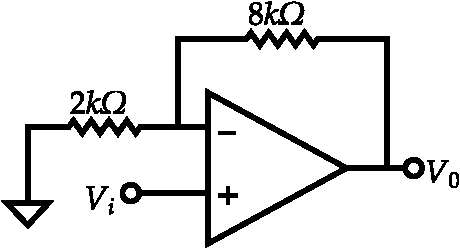
\includegraphics[height=2.8cm,width=5cm]{CE-2}
	\end{figure}
	 \begin{tasks}(4)
		\task[\textbf{a.}]20
		\task[\textbf{b.}]$4.5$
		\task[\textbf{c.}]4
		\task[\textbf{d.}] 5
	\end{tasks}
	\begin{answer}
		$$
		\begin{aligned}
		&\text { A closed loop gain, }\\
		A_{C L}&=\frac{V_{0}}{V_{i}}=\frac{A_{o d}}{1+\beta A_{o d}}, \beta=\frac{2 K}{8 K+2 K}=0.2, A_{C L}=\frac{45}{1+(45)(0.2)}=4.5
	\end{aligned}
	$$
	So the corrext answer is \textbf{Option (b)}
	\end{answer}
	\item  The circuit shown below uses only NAND gates. Find the final output. 
	\begin{figure}[H]
		\centering
		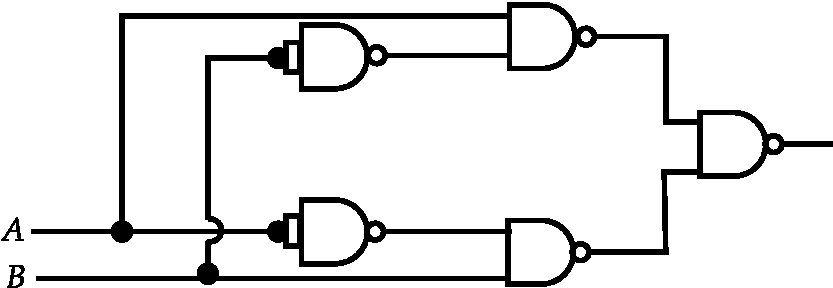
\includegraphics[height=2.8cm,width=8cm]{CE-3}
	\end{figure}
	 \begin{tasks}(4)
		\task[\textbf{a.}]A XOR B
		\task[\textbf{b.}]$\mathrm{AOR} \mathrm{B}$
		\task[\textbf{c.}]A AND B
		\task[\textbf{d.}] A NOR B
	\end{tasks}
	\begin{answer}$\left. \right. $\\
		\begin{figure}[H]
			\centering
			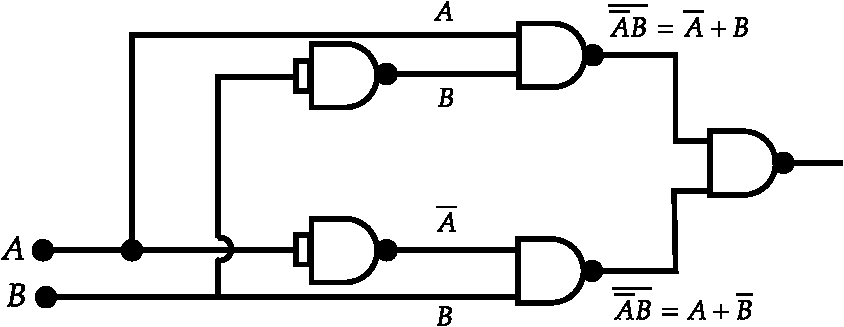
\includegraphics[height=3.3cm,width=8cm]{CE-4}
		\end{figure}
		$$
		\begin{aligned}
		\overline{(\bar{A}+B) \cdot(A+\bar{B})}=\overline{\bar{A}+B}+\overline{A+\bar{B}}=A \bar{B}+\bar{A} B=A X O R B
	\end{aligned}
	$$
		So the corrext answer is \textbf{Option (a)}
	\end{answer}
	\item In a digital circuit for three input signals $(A, B$ and $C)$ the final output $(Y)$ should be such that for inputs\\\\
	\begin{tabular}{lll}
		$\mathrm{A}$ & $\mathrm{B}$ & $\mathrm{C}$ \\
		\hline 0 & 0 & 0 \\
		0 & 0 & 1 \\
		0 & 1 & 0 \\
		\hline
	\end{tabular}\\\\
	the output (Y) should be low and for all other cases it should be high. Which of the following digital circuits will give such output ?
	 \begin{tasks}(2)
		\task[\textbf{a.}]\begin{figure}[H]
			\centering
			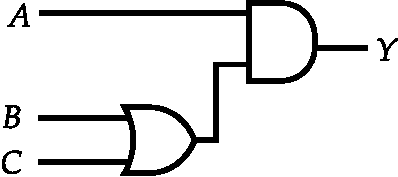
\includegraphics[height=1.7cm,width=4cm]{CE-5}
		\end{figure}
		\task[\textbf{b.}]\begin{figure}[H]
			\centering
			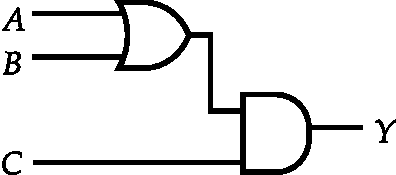
\includegraphics[height=1.7cm,width=4cm]{CE-6}
		\end{figure}
		\task[\textbf{c.}]\begin{figure}[H]
			\centering
			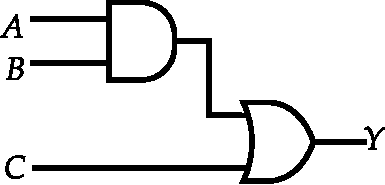
\includegraphics[height=1.7cm,width=4cm]{CE-7}
		\end{figure}
		\task[\textbf{d.}] \begin{figure}[H]
			\centering
			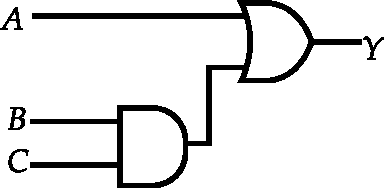
\includegraphics[height=1.7cm,width=4cm]{CE-8}
		\end{figure}
	\end{tasks}
	\begin{answer}
		$$
		\begin{aligned}
		\begin{array}{c|ccc}
		A & B & C & y \\
		\hline 0 & 0 & 0 & 0 \\
		0 & 0 & 1 & 0 \\
		0 & 1 & 0 & 0 \\
		1 & 0 & 0 & 1
		\end{array}
	\end{aligned}
	$$
	Only option (d) will give such output.\\
		So the corrext answer is \textbf{Option (d)}
	\end{answer}
	\item The mean kinetic energy of the conduction electrons in metals is ordinary much higher than $k T$ because
	 \begin{tasks}(1)
		\task[\textbf{a.}]Electrons have many more degrees of freedom than atoms do
		\task[\textbf{b.}] The electrons and the lattice are not in thermal equilibrium
		\task[\textbf{c.}]The electrons form a degenerate Fermi gas
		\task[\textbf{d.}] Electrons in metals are highly relativistic
	\end{tasks}
\begin{answer}
	The mean kinetic energy of the conduction electrons in metal is ordinary much higher than $\mathrm{kT}$ because the electrons form a degenerate fermi gas.\\
		So the corrext answer is \textbf{Option (c)}
\end{answer}
\item Which of the following statements concerning the electrical conductivities at room temperature of a pure copper sample and a pure silicon sample is NOT true ?
	[BHU 2012]
	 \begin{tasks}(1)
		\task[\textbf{a.}]If the temperature of the copper sample is increased, its conductivity will decrease
		\task[\textbf{b.}]If the temperature of the silicon sample is increased, its conductivity will increase
		\task[\textbf{c.}] The addition of an impurity in the copper sample always decreases its conductivity
		\task[\textbf{d.}]  The addition of an impurity in the silicon always decreases its conductivity
	\end{tasks}
\begin{answer}
		Out of above options, the option (d) "The addition of an impurity in the silicon always decreases its conductivity" is not type.\\
	So the corrext answer is \textbf{Option (d)}
\end{answer}
\item Indicate the statement about the semiconductors which is false ?
 \begin{tasks}(1)
	\task[\textbf{a.}] $n$-type semiconductors are obtained by doping phosphorus into silicon
	\task[\textbf{b.}]The conductivity of all semiconductors always increases with temperature
	\task[\textbf{c.}]$p$-type semiconductors are obtained by doping boron into silicon
	\task[\textbf{d.}] Intrinsic semiconductors are insulators at $T=0{ }^{\circ} \mathrm{K}$
\end{tasks}
\begin{answer}
Out of the above options, the option (b) the conductivity of all semiconductors always increases with temperature is false.\\
	So the corrext answer is \textbf{Option (b)}
\end{answer}
	\item Which of the following statements is true about the effective mass of electron in crystal?
	 \begin{tasks}(1)
		\task[\textbf{a.}]It is positive near the top of energy band 
		\task[\textbf{b.}]It is negative near the bottom of energy band
		\task[\textbf{c.}]It is constant through out the band
		\task[\textbf{d.}] It is negative near the top of energy band
	\end{tasks}
	\begin{answer}
	Out of the above options, "It is negative near the top of energy band"' is correct.
	So the corrext answer is \textbf{Option (d)}
	\end{answer}
\item Electrical conductivity of insulators is in the range:
	 \begin{tasks}(2)
		\task[\textbf{a.}]$10^{-10}(\Omega-\mathrm{mm})^{-1}$
		\task[\textbf{b.}]$10^{-10}(\Omega-\mathrm{cm})^{-1}$
		\task[\textbf{c.}] $10^{-10}(\Omega-\mathrm{m})^{-1}$
		\task[\textbf{d.}] $10^{-8}(\Omega-\mathrm{m})^{-1}$
	\end{tasks}
	\begin{answer}
	Electrical conductivity of intensity is in the range $10^{-8}(\Omega-\mathrm{m})^{-1}$. \\
	So the corrext answer is \textbf{Option (d)}
	\end{answer}
	\item Energy band gap size for semiconductors is in the ranges
	 \begin{tasks}(2)
		\task[\textbf{a.}]$1-2 \mathrm{eV}$
		\task[\textbf{b.}]$2-3 \mathrm{eV}$
		\task[\textbf{c.}]$3-4 \mathrm{eV}$
		\task[\textbf{d.}]  greater than $4 \mathrm{eV}$
	\end{tasks}
	\begin{answer}
	Energy band gap size for semiconductors is in the ranges $1-2 \mathrm{eV}$. \\
	So the corrext answer is \textbf{Option (a)}
	\end{answer}
	\item Fermi energy level for intrinsic semiconductors lies :
	 \begin{tasks}(2)
		\task[\textbf{a.}]At the middle of the band gap
		\task[\textbf{b.}]Close to the conduction band
		\task[\textbf{c.}]Close to valence band
		\task[\textbf{d.}] Inside valence band
	\end{tasks}
	\begin{answer}
		Fermi-level for intrinsic semiconductors lies at the middle of the band gap. \\
		So the corrext answer is \textbf{Option (a)}
	\end{answer}
	\item Indicate the false statement about the semiconductors
	 \begin{tasks}(1)
		\task[\textbf{a.}]All intrinsic semiconductors are insulators at $\mathrm{T}=0^{\circ} \mathrm{K}$
		\task[\textbf{b.}]At very high temperature all semiconductors become intrinsic semiconductors
		\task[\textbf{c.}] The conductivity of all semiconductors always increases with temperature
		\task[\textbf{d.}] N-type semiconductors are obtained by doping phosphorus into silicon
	\end{tasks}
	\begin{answer}
			Out of the given options, the option (c) the conductivity of all semiconductors always increases with temperature.\\
		So the corrext answer is \textbf{Option (c)}
	\end{answer}
\item The reverse saturation current in germanium $p-n$ diode is of the order of
	 \begin{tasks}(4)
		\task[\textbf{a.}]$n \mathrm{~A}$
		\task[\textbf{b.}]$\mu \mathrm{A}$
		\task[\textbf{c.}] $\mathrm{mA}$
		\task[\textbf{d.}] Ampere
	\end{tasks}
	\begin{answer}
	The reverse saturation current in germanium $p-n$ junction diode is of the order of microampere ( $\mu \mathrm{A})$\\
		So the corrext answer is \textbf{Option (a)}
	\end{answer}
\item The Fermi level in an $n$-type semiconductor at $0{ }^{\circ} \mathrm{K}$
 \begin{tasks}(1)
	\task[\textbf{a.}]Lies below the donor level
	\task[\textbf{b.}]Lies in the conduction band
	\task[\textbf{c.}]Lies half-way between the conduction band and donor level
	\task[\textbf{d.}] Coincides with the intrinsic Fermi level
\end{tasks}
\begin{answer}
	The Fermilevel in an $n$-type semiconductor at $0{ }^{\circ} \mathrm{K}$ lies half-way between the conduction band and donor level.\\
	So the corrext answer is \textbf{Option (c)}
\end{answer}
\item If the Fermi energy of a metal at $0{ }^{\circ} \mathrm{K}, 10 \mathrm{eV}$, the mean energy of the electrons in the metal at $0{ }^{\circ} \mathrm{K}$ is
 \begin{tasks}(4)
	\task[\textbf{a.}]$6 \mathrm{eV}$
	\task[\textbf{b.}] $5 \mathrm{eV}$
	\task[\textbf{c.}]$1.5 \mathrm{eV}$
	\task[\textbf{d.}]  $2 \mathrm{eV}$
\end{tasks}
\begin{answer}
	$$
	\begin{aligned}
		&\text { The average energy of electrons in the metal at } 0{ }^{\circ} \mathrm{K} \text {, }\\
		\vec{E}&=\frac{3}{5} E_{f}=\frac{3}{5} \times 10 \mathrm{eV}=6 \mathrm{eV}
\end{aligned}
$$
	So the corrext answer is \textbf{Option (a)}
\end{answer}
\item Consider the speed of gas molecules in a container. The ratio of speeds of the gas molecules at $27^{\circ} \mathrm{C}$ to that at $-73^{\circ} \mathrm{C}$ is
 \begin{tasks}(4)
	\task[\textbf{a.}]$\sqrt{\frac{3}{2}}$
	\task[\textbf{b.}]$\sqrt{\frac{2}{3}}$
	\task[\textbf{c.}] $\sqrt{3}$
	\task[\textbf{d.}] $\sqrt{\frac{1}{3}}$
\end{tasks}
\begin{answer}
	$$
	\begin{aligned}
	V \propto \sqrt{T} \text { where } T \text { is temperature in Kelvin }\\
	\text { Ratio of speeds }=\frac{\sqrt{300}}{\sqrt{200}}=\sqrt{\frac{3}{2}}
\end{aligned}
$$
	So the corrext answer is \textbf{Option (a)}
\end{answer}
\item Two identical bodies have internal energy $U=N C T$, with $N$ and $C$ the same for each body. The initial temperatures of the bodies are $T_{1}$ and $T_{2}$, and they are used as a source of work by connecting them to a Carnot heat engine and bringing them to a common final temperature $T_{f}$ which is
 \begin{tasks}(4)
	\task[\textbf{a.}]$T_{1}^{2} / T_{2}$
	\task[\textbf{b.}]$\sqrt{T_{1} T_{2}}$
	\task[\textbf{c.}]$T_{2}^{2} / T_{1}$
	\task[\textbf{d.}] $\left(T_{1}+T_{2}\right) / 2$
\end{tasks}
\begin{answer}
		So the corrext answer is \textbf{Option (b)}
\end{answer}
\item A monatomic ideal gas of $N$ atoms undergoes isothermal reversible expansion from volume $V_{1}$ to $V_{2}$. The change in entropy of the gas is
 \begin{tasks}(2)
	\task[\textbf{a.}]0
	\task[\textbf{b.}]$\quad N k_{B} \ln \frac{V_{1}}{V_{2}}$
	\task[\textbf{c.}] $2 N k_{B} \ln \frac{V_{2}}{V_{1}}$
	\task[\textbf{d.}]  $\quad N k_{B} \ln \frac{V_{2}}{V_{1}}$
\end{tasks}
\begin{answer}
	$$
	\begin{aligned}
	\text { Change in entropy }\\
	\Delta S &=\int \frac{d Q}{T} \\
	&=\int \frac{d W}{T}\\
	\text { (For isothermal process } d Q&=d W \text { ) }\\
	&=\int \frac{P}{T} d V \\
	&=n R \int_{V_{1}}^{V_{2}} \frac{d V}{V} \\
	&=\frac{N}{N_{0}} R \ln \frac{V_{2}}{V_{1}} \\
	&=N k_{B} \ln \frac{V_{2}}{V_{1}}
\end{aligned}
$$
	So the corrext answer is \textbf{Option (d)}
\end{answer}
\item Keeping density and sound speed constant, doubling the pressure implies that the ratio of specific heats $C_{p} / C_{v}$
 \begin{tasks}(2)
	\task[\textbf{a.}]Doubles
	\task[\textbf{b.}]Halves
	\task[\textbf{c.}]Remains constant
	\task[\textbf{d.}]Quadruples
\end{tasks}
\begin{answer}
	$$
	\begin{aligned}
	\text{Velocity }\quad &V=\sqrt{\frac{\gamma P}{\rho}} \\
	&\gamma=\frac{\rho V^{2}}{P}
\end{aligned}
$$
Keeping $\rho$ and $V$ same and doubling pressure will halves $\gamma$.\\
So the corrext answer is \textbf{Option (b)}
\end{answer}
\item A rigid triangular molecule consists of three non-collinear atoms joined by rigid rods. The constant pressure molar specific heat $\left(C_{p}\right)$ of an ideal gas consisting of such moecules is
 \begin{tasks}(4)
	\task[\textbf{a.}] $6 R$
	\task[\textbf{b.}]$5 R$
	\task[\textbf{c.}] $4 R$
	\task[\textbf{d.}] $3 R$
\end{tasks}
\begin{answer}
	$$
	\begin{aligned}
	C_{v}&=\frac{f R}{2}\\
\text{	where $f$ }&\text{is degree of freedom
	For rigid triangular molecule, $f=6$}\\
\text{So,}\quad 
&C_{v}=3 R \\
&C_{p}=C_{v}+R=4 R
\end{aligned}
$$
So the corrext answer is \textbf{Option (c)}
\end{answer}
\item If $\mathrm{U}, \mathrm{F}, \mathrm{H}$, and $\mathrm{G}$ represent internal energy, Helmholtz free energy, enthalpy, and Gibbs free energy
respectively, then which one of the following is a correct thermodynamic relation?
 \begin{tasks}(2)
	\task[\textbf{a.}]$d U=P d V-T d S$
	\task[\textbf{b.}] $d H=V d P+T d S$
	\task[\textbf{c.}]$d F=-P d V+S d T$
	\task[\textbf{d.}]  $d G=V d P+S d T$
\end{tasks}
\begin{answer}
	$$
	\begin{aligned}
	d U &=T d S-P d V \\
	H &=U+P V \\
	d H &=d U+P d V+V d P \\
	&=T d S-p d V+P d V+V d P \\
	&=T d S+V d P
\end{aligned}
$$
So the corrext answer is \textbf{Option (b)}
\end{answer}
\item The molar specific heat of a gas as given from the kinetic theory is $\frac{5}{2} R$. If it is not specified whether it is $C_{p}$ or $C_{r}$ one could conclude that the molecules of the gas
 \begin{tasks}(1)
	\task[\textbf{a.}]Are definitely monatomic
	\task[\textbf{b.}]Are definitely rigid diatomic
	\task[\textbf{c.}]Are definitely non-rigid diatomic
	\task[\textbf{d.}]Can be monatomic or rigid diatomic
\end{tasks}
\begin{answer}
So the corrext answer is \textbf{Option (d)}
\end{answer}
\item The value of entropy at absolute zero of temperature would be
 \begin{tasks}(1)
	\task[\textbf{a.}]Zero for all the materials
	\task[\textbf{b.}]Finite for all the materials
	\task[\textbf{c.}]Zero for some materials and non-zero for others
	\task[\textbf{d.}] Unpredictable for any material
\end{tasks}
\begin{answer}
So the corrext answer is \textbf{Option (a)}
\end{answer}
\item Experimental measurements of heat capacity per $\mathrm{m}_{0 l_{e}}$ of Aluminium at low temperatures show that the data can be fitted to the formula, $C_{V}=a T+b T^{3}$, where $a=0.00135 \mathrm{JK}^{-2} \mathrm{~mole}^{-1}, b=2.48 \times 10^{-5} \mathrm{JK}^{-4}$ mole-l and $T$ is the temperature in Kelvin. The entropy of mole of Aluminium at such temperatures is given by the formula
 \begin{tasks}(1)
	\task[\textbf{a.}]$a T+\frac{b}{3} T^{3}+c$, where $c>0$ is a constant
	\task[\textbf{b.}]$\frac{a T}{2}+\frac{b}{4} T^{3}+c$, where $c>0$ is a constant
	\task[\textbf{c.}]$a T+\frac{b}{3} T^{3}$
	\task[\textbf{d.}] $\frac{a T}{2}+\frac{b}{4} T^{3}$
\end{tasks}
\begin{answer}
	$$
	\begin{aligned}
	\Delta S &=\int \frac{d Q}{T}=\int \frac{C_{V} d T}{T} \\
	&=\int\left(a+b T^{2}\right) d T \\
	&=a T+\frac{b T^{3}}{3}+c
\end{aligned}
$$
So the corrext answer is \textbf{Option (a)}
\end{answer}
\item A thermodynamic system is maintained at constant temperature and pressure. In thermodynamic equilibrium, its
 \begin{tasks}(1)
	\task[\textbf{a.}]Gibbs free energy is minimum
	\task[\textbf{b.}]Enthalpy is maximum
	\task[\textbf{c.}]Helmholtz free energy is minimum
	\task[\textbf{d.}]Internal energy is zero
\end{tasks}
\begin{answer}
So the corrext answer is \textbf{Option (a)}
\end{answer}
\item A gas of molecular mass $m$ is at temperature $T$. If the gas obeys Maxwell-Boltzmann velocity distribution, the average speed of molecules is given by
 \begin{tasks}(4)
	\task[\textbf{a.}]$\sqrt{\frac{k_{B} T}{m}}$
	\task[\textbf{b.}]$\sqrt{\frac{2 k_{B} T}{m}}$
	\task[\textbf{c.}]$\sqrt{\frac{2 k_{B} T}{\pi m}}$
	\task[\textbf{d.}] $\sqrt{\frac{8 k_{B} T}{\pi m}}$
\end{tasks}
\begin{answer}
	So the corrext answer is \textbf{Option (d)}
\end{answer}
\item In 1 -dimension, an ensemble of $N$ classical particles has energy of the form $E=\frac{P_{x}^{2}}{2 m}+\frac{1}{2} k x^{2}$. The average internal energy of the system at temperature $T$ is
 \begin{tasks}(4)
	\task[\textbf{a.}]$\frac{3}{2} N k_{B} T$
	\task[\textbf{b.}]$\frac{1}{2} N k_{B} T$
	\task[\textbf{c.}]$3 N k_{B} T$
	\task[\textbf{d.}] $N k_{B} T$
\end{tasks}
\begin{answer}
	So the corrext answer is \textbf{Option (d)}
\end{answer}
\item The root mean square speed of an ideal gas, made up of molecules of molecular weight $0.0831 \mathrm{~kg} / \mathrm{mol}$, at temperature $300 \mathrm{~K}$ is (Take universal gas constant $R=8.31 \mathrm{~J} / \mathrm{mol} \mathrm{} K$ )
 \begin{tasks}(4)
	\task[\textbf{a.}] $100 \mathrm{~m} / \mathrm{s}$
	\task[\textbf{b.}]$200 \mathrm{~m} / \mathrm{s}$
	\task[\textbf{c.}] $300 \mathrm{~m} / \mathrm{s}$
	\task[\textbf{d.}]  $400 \mathrm{~m} / \mathrm{s}$
\end{tasks}
\begin{answer}
	$$
	\begin{aligned}
	V_{r m s} &=\sqrt{\frac{3 R T}{M}} \\
	&=\sqrt{\frac{3 \times 8.31 \times 300}{0.0831}}=300 \mathrm{~m} / \mathrm{s}\\
	E&=7 \times \frac{1}{2} k T=\frac{7}{2} k T
\end{aligned}
$$
	So the corrext answer is \textbf{Option (c)}
\end{answer}
\item In a diatomic gas system, molecules are free to translate, rotate and vibrate. The average kinetic energy per molecule is
 \begin{tasks}(4)
	\task[\textbf{a.}] $\frac{1}{2} k T$
	\task[\textbf{b.}]$\frac{3}{2} k T$
	\task[\textbf{c.}]$\frac{5}{2} k T$
	\task[\textbf{d.}]  $\frac{7}{2} k T$
\end{tasks}
\begin{answer}
	$$
	\begin{aligned}
	&\text { The degree of freedom } n=7\\
	&\text { According to law of equipartition of energy }\\
	E&=7 \times \frac{1}{2} k T=\frac{7}{2} k T
\end{aligned}
$$
	So the corrext answer is \textbf{Option (d)}
\end{answer}
\item In Kinetic theory of gases, the pressure of gas in a container container can be written as $p=\frac{2}{3} U$. For a monatomic gas, the quantity $U$ is
 \begin{tasks}(1)
	\task[\textbf{a.}]Kinetic energy per molecule
	\task[\textbf{b.}]Total kinetic energy of all the molecules in the container
	\task[\textbf{c.}]Total average kinetic energy of molecules in one mole
	\task[\textbf{d.}] Total average kinetic energy of molecules in unit volume.
\end{tasks}
\begin{answer}
		So the correct answer is \textbf{Option (d)}
\end{answer}
\end{enumerate}